\documentclass[a4paper]{fhnwreport} %Legt grundlegende Formatierungen wie 
\usepackage{amssymb}
\graphicspath{{./graphics/}}%Change according to graphics folder!

\title{Pflichtenheft SolarMeasurementSystem}
\date{Windisch, \today}

\begin{document}

\maketitle

\vspace*{2cm}

\vfill
\textsc{
\begin{tabbing}
Auftraggeber: \hspace{4em} \=   Hans Gysin \\[2ex]
Fachcoaches:  \>  Matthias Meier \\ \> Pascal Schleuniger \\ \> Hans Gysin \\ \> Anita Gertiser \\ \>Pascal Buchschacher \\ \>Bonnie Domenghino\\[2ex]
Gruppe:  \>  FS15 pro2E Team 3 \\[2ex]
Teammitglieder:  \> David Laim (Projektleiter) \\ \> Sarah Simmen (Stv. Projektleiterin) \\ \> Anita Rosenberger \\ \> Claudius J"org \\ \> Denis Stampfli \\ \>Simon Sturm \\ \>Yohannes Measho \\[2ex]
Studiengang: \> Elektro- und Informationstechnik
\end{tabbing}}
\vfill
\hbox{}
\clearpage

\tableofcontents 
\clearpage

\section{Projektorganisation}
\section{Projektplanung}

Zur besseren Einteilung der Ressourcen und um den reibungslosen Projektablauf sicherzustellen wurde ein Projektplan (Abbildung \ref{fig::Ereignisse}) erstellt. 
Dabei wurde darauf geachtet, dass die Arbeitsbelastung im Team gleichmässig aufgeteilt wird.\\
Dieser ist im Anhang (Abbildung \ref{fig::Projektplanung_1}) im Grossformat ersichtlich.


\begin{figure}[h] 
\centering
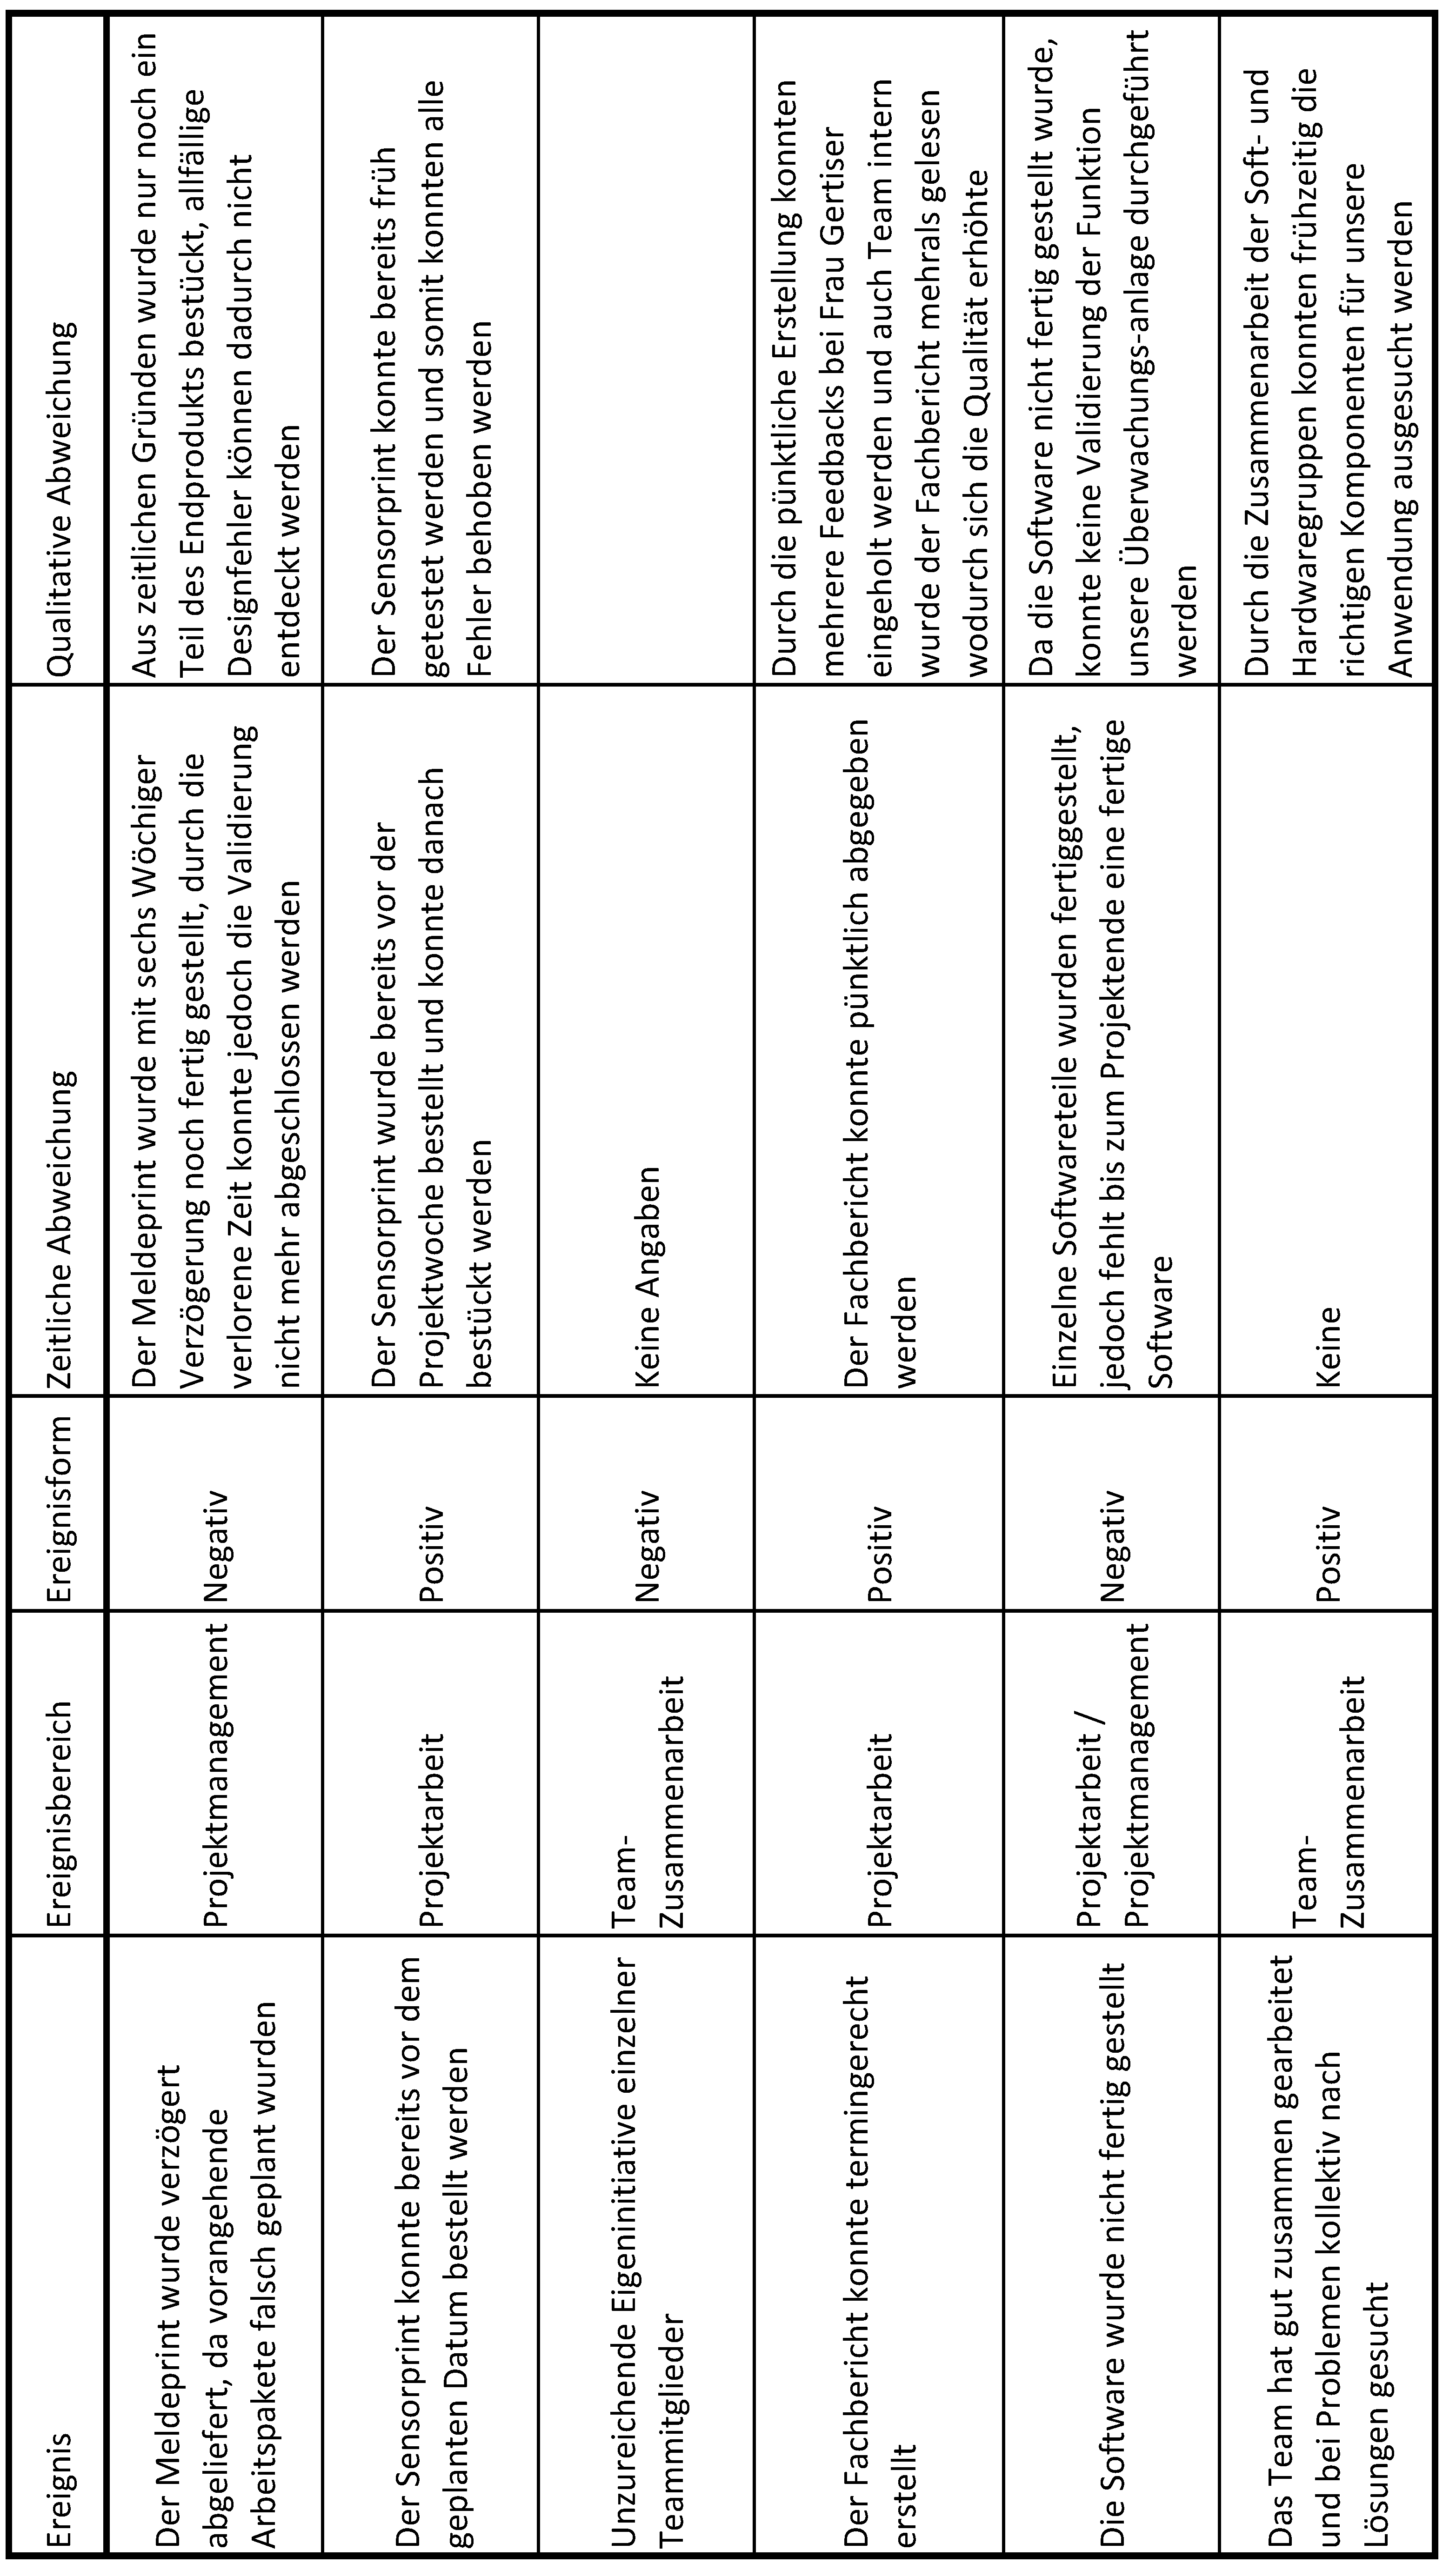
\includegraphics[width=0.77\textwidth]{graphics/Ereignisse.png}%
\caption{Ereignisse}%
\label{fig::Ereignisse}%
\end{figure}
\section{Projektbudget}

Das Projektbudget bezieht sich auf die vorgesehenen Arbeitsstunden. Die Projektmanagement-Stunden werden mit 148 Sfr. verrechnet, die restlichen mit 74 SFr. In Abbildung \ref{fig::Budget_1} wird die Kostenaufstellung gezeigt und in Abbildung \ref{fig::Budget_2} die Kostenverteilung.


\begin{figure}[h] 
\centering
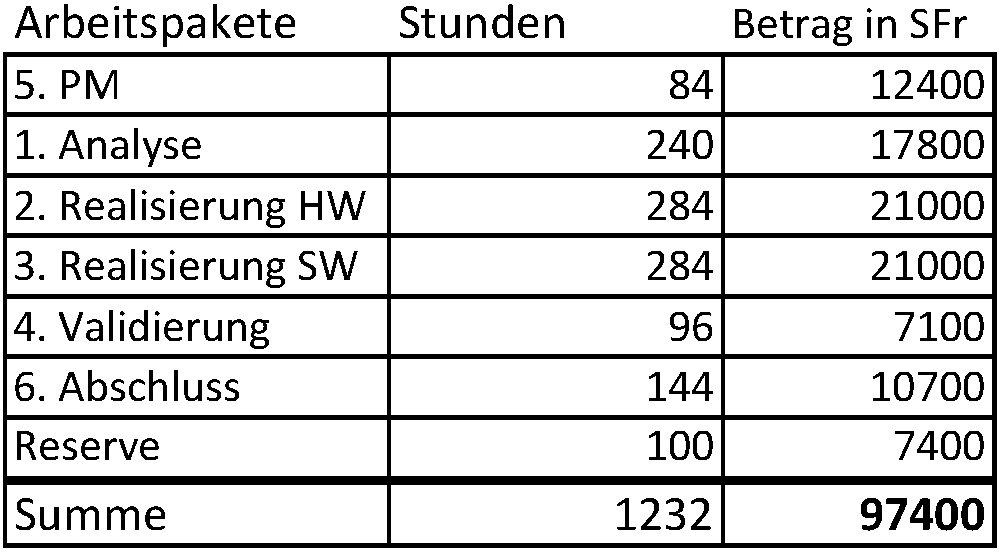
\includegraphics[width=0.6\textwidth]{Budget_1.png}%
\caption{Kostenaufstellung}%
\label{fig::Budget_1}%
\end{figure}

\begin{figure}[h] 
\centering
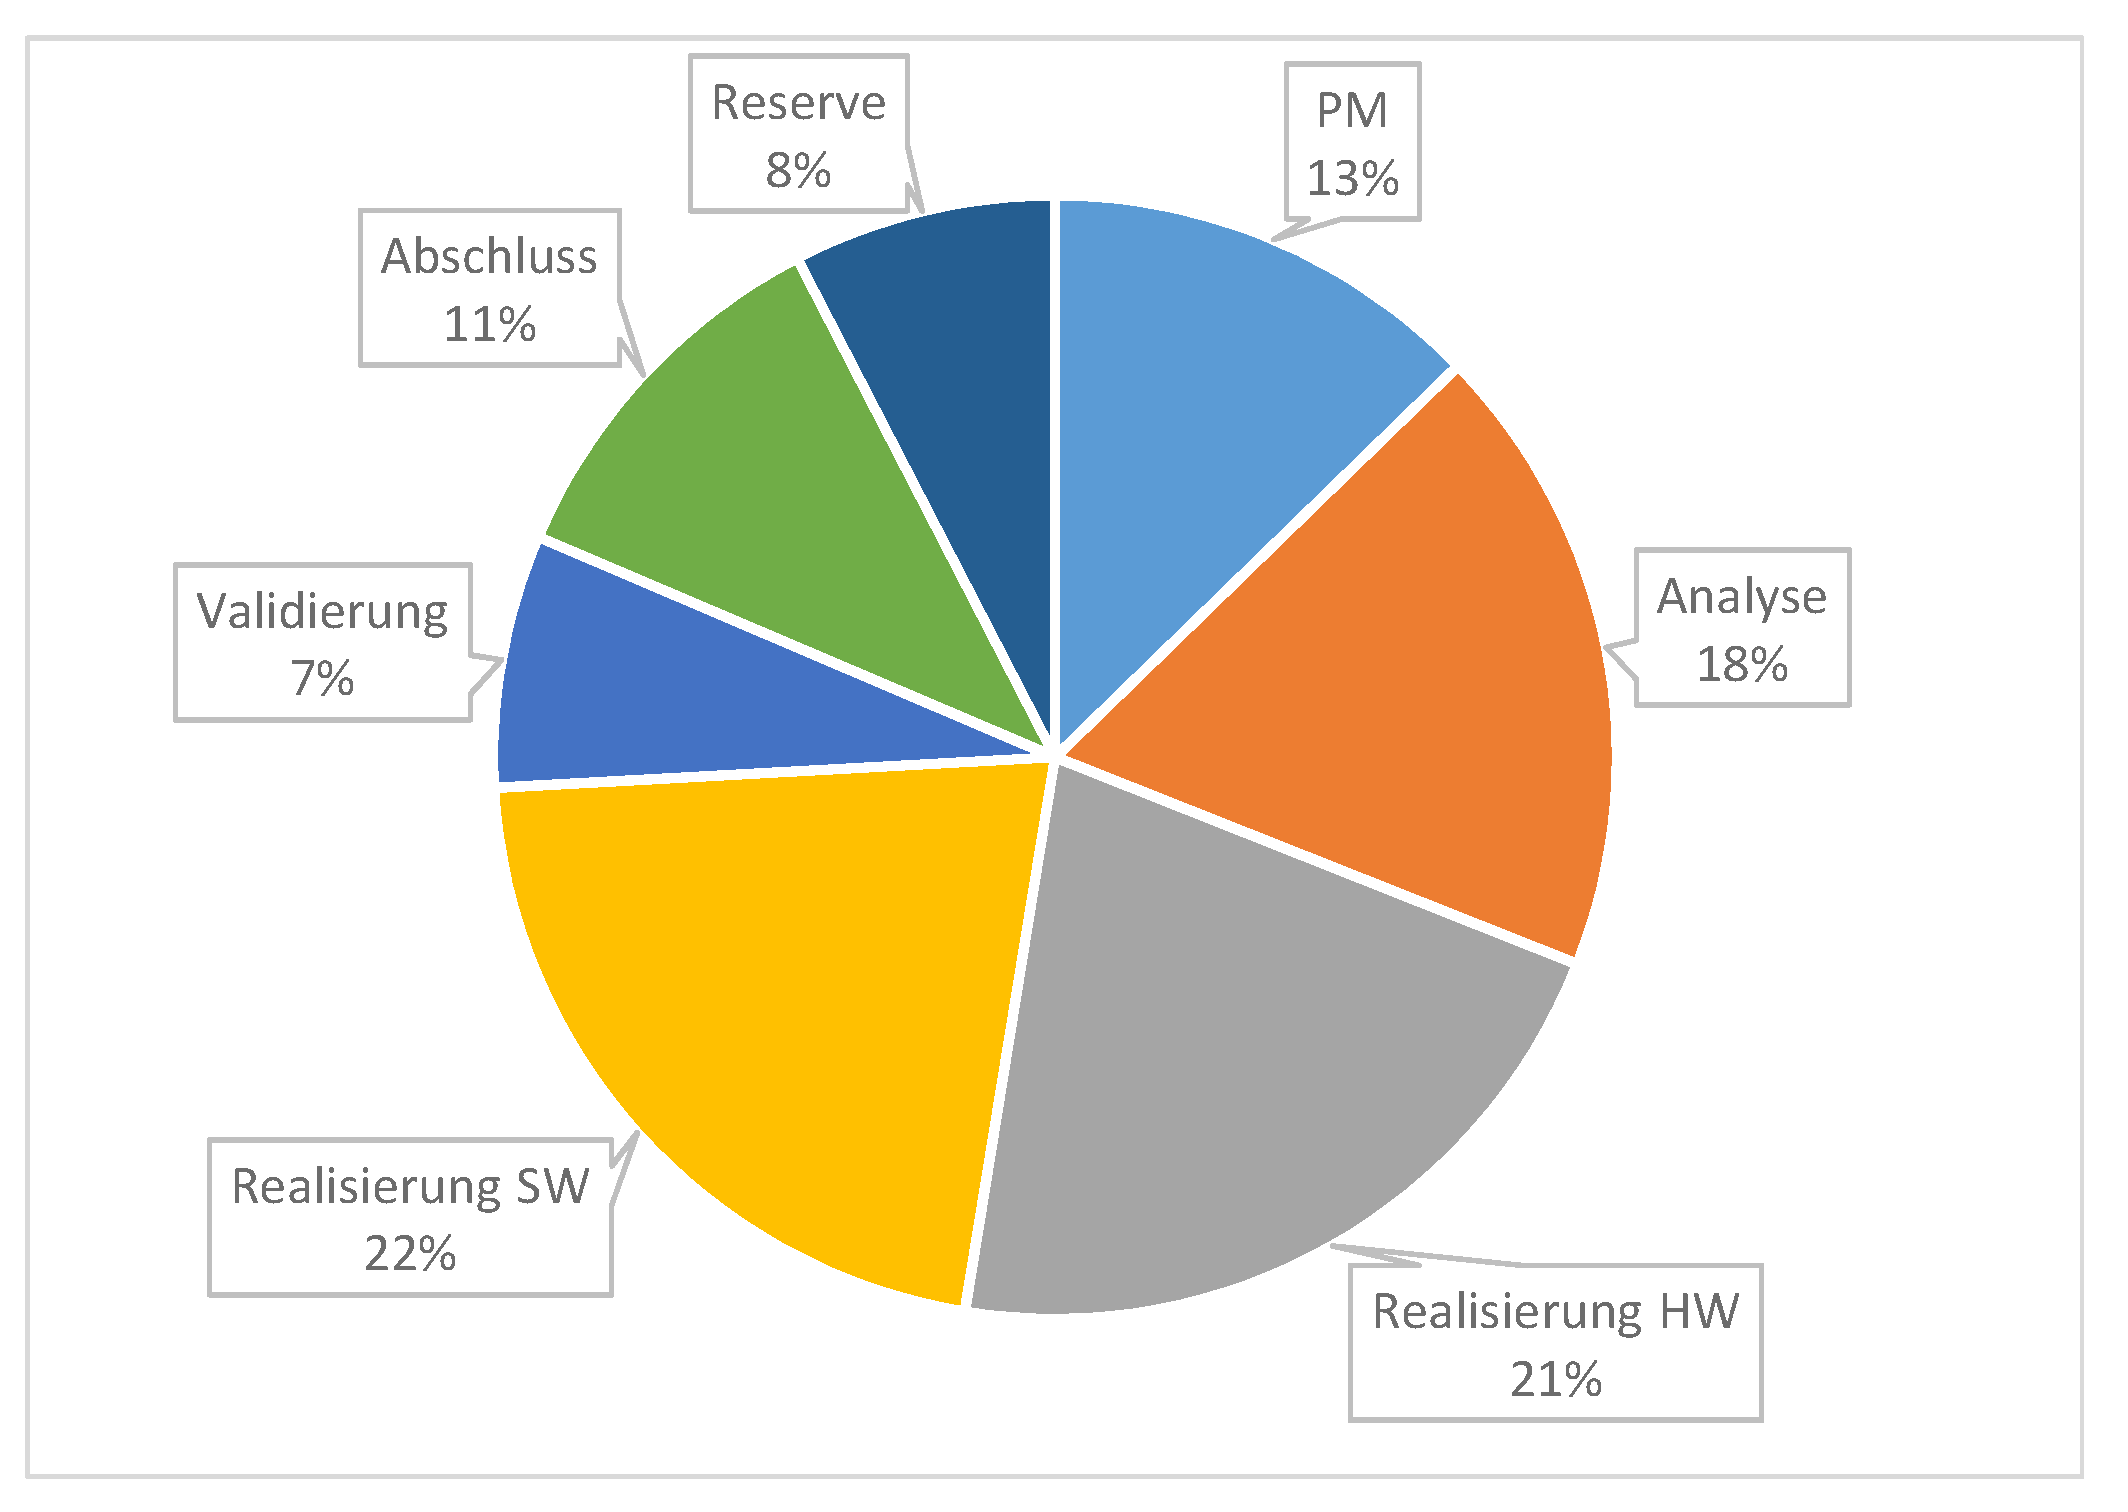
\includegraphics[width=0.8\textwidth]{Budget_2.png}%
\caption{Kostenverteilung}%
\label{fig::Budget_2}%
\end{figure}

Die Materialkosten können zu diesem Zeitpunkt noch nicht abgeschätzt werden, jedoch sollte das maximale Budget für den Materialeinkauf von 250 Franken nicht überschritten werden.
\section{Kommunikation}


\section{Risikomanagement}

Das Projekt verläuft während einer langen Zeit und beansprucht grosse Ressourcen. Es ist daher wichtig, dass Risiken frühzeitig erkannt werden und auch bestmöglich verhindert werden. In der folgenden Abbildung \ref{fig::Risikomanagement} ist das detaillierte Risikomanagement ersichtlich.


\begin{figure}[h] 
\centering
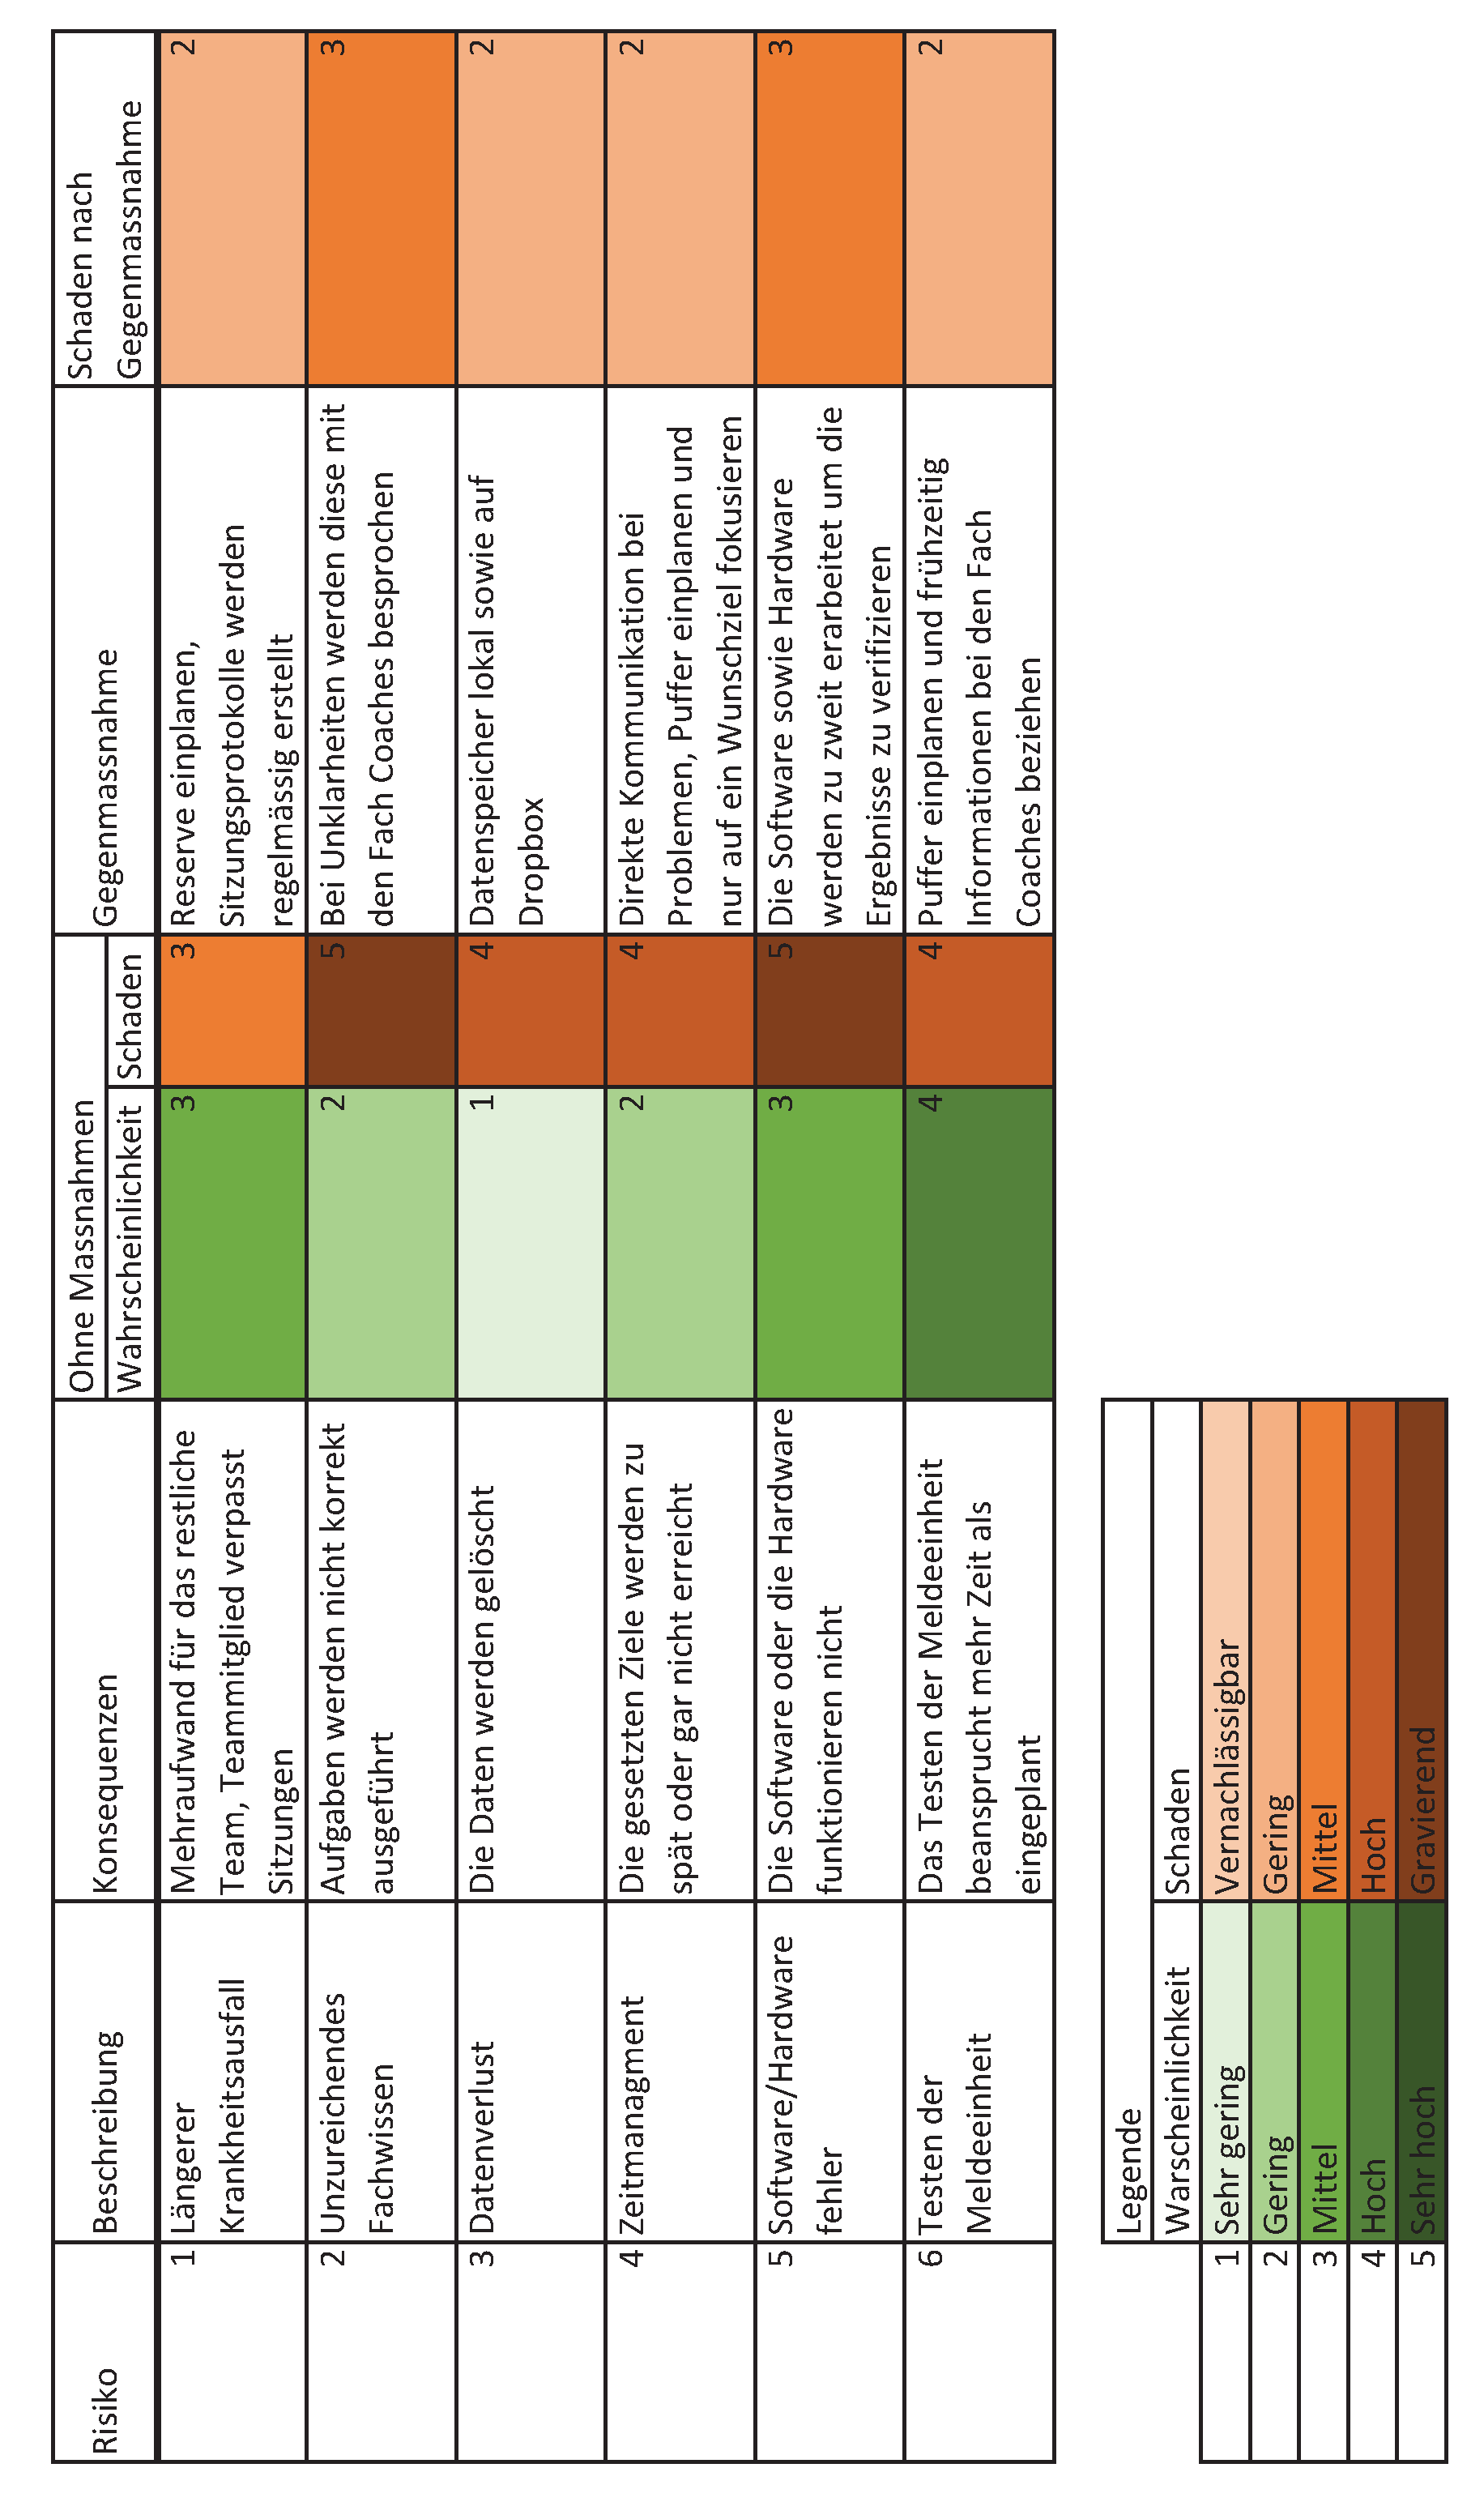
\includegraphics[width=0.65\textwidth]{Risikomanagment.png}%
\caption{Risikomanagement}%
\label{fig::Risikomanagement}%
\end{figure}
\section{Projektvereinbarung}

$\square$ Projekt wird genehmigt.\\
$\square$ Projekt wird nicht genehmigt.\\
\begin{tabbing}
\textbf{Hans Gysin, Auftraggeber} \\[3ex]
\noindent\rule{0.4\textwidth}{1pt} \hspace{6em} \=  \noindent\rule{0.4\textwidth}{1pt} \\ Ort, Datum \> Unterschrift \\[2ex] 

\textbf{David Laim, Projektleiter} \\[3ex]
\noindent\rule{0.4\textwidth}{1pt} \>  \noindent\rule{0.4\textwidth}{1pt} \\ Ort, Datum \> Unterschrift \\[2ex]

\textbf{Anita Rosenberger} \\[3ex]
\noindent\rule{0.4\textwidth}{1pt} \>  \noindent\rule{0.4\textwidth}{1pt} \\ Ort, Datum \> Unterschrift \\[2ex]

\textbf{Claudius J"org} \\[3ex]
\noindent\rule{0.4\textwidth}{1pt} \>  \noindent\rule{0.4\textwidth}{1pt} \\ Ort, Datum \> Unterschrift \\[2ex]

\textbf{Sarah Simmen} \\[3ex]
\noindent\rule{0.4\textwidth}{1pt} \>  \noindent\rule{0.4\textwidth}{1pt} \\ Ort, Datum \> Unterschrift \\[2ex]

\textbf{Yohannes Measho} \\[3ex]
\noindent\rule{0.4\textwidth}{1pt} \>  \noindent\rule{0.4\textwidth}{1pt} \\ Ort, Datum \> Unterschrift \\[2ex]

\textbf{Simon Sturm} \\[3ex]
\noindent\rule{0.4\textwidth}{1pt} \>  \noindent\rule{0.4\textwidth}{1pt} \\ Ort, Datum \> Unterschrift \\[2ex]

\textbf{Denis Stampfli} \\[3ex]
\noindent\rule{0.4\textwidth}{1pt} \>  \noindent\rule{0.4\textwidth}{1pt} \\ Ort, Datum \> Unterschrift \\[2ex]

\end{tabbing}


\end{document}









